\section{Implementation}
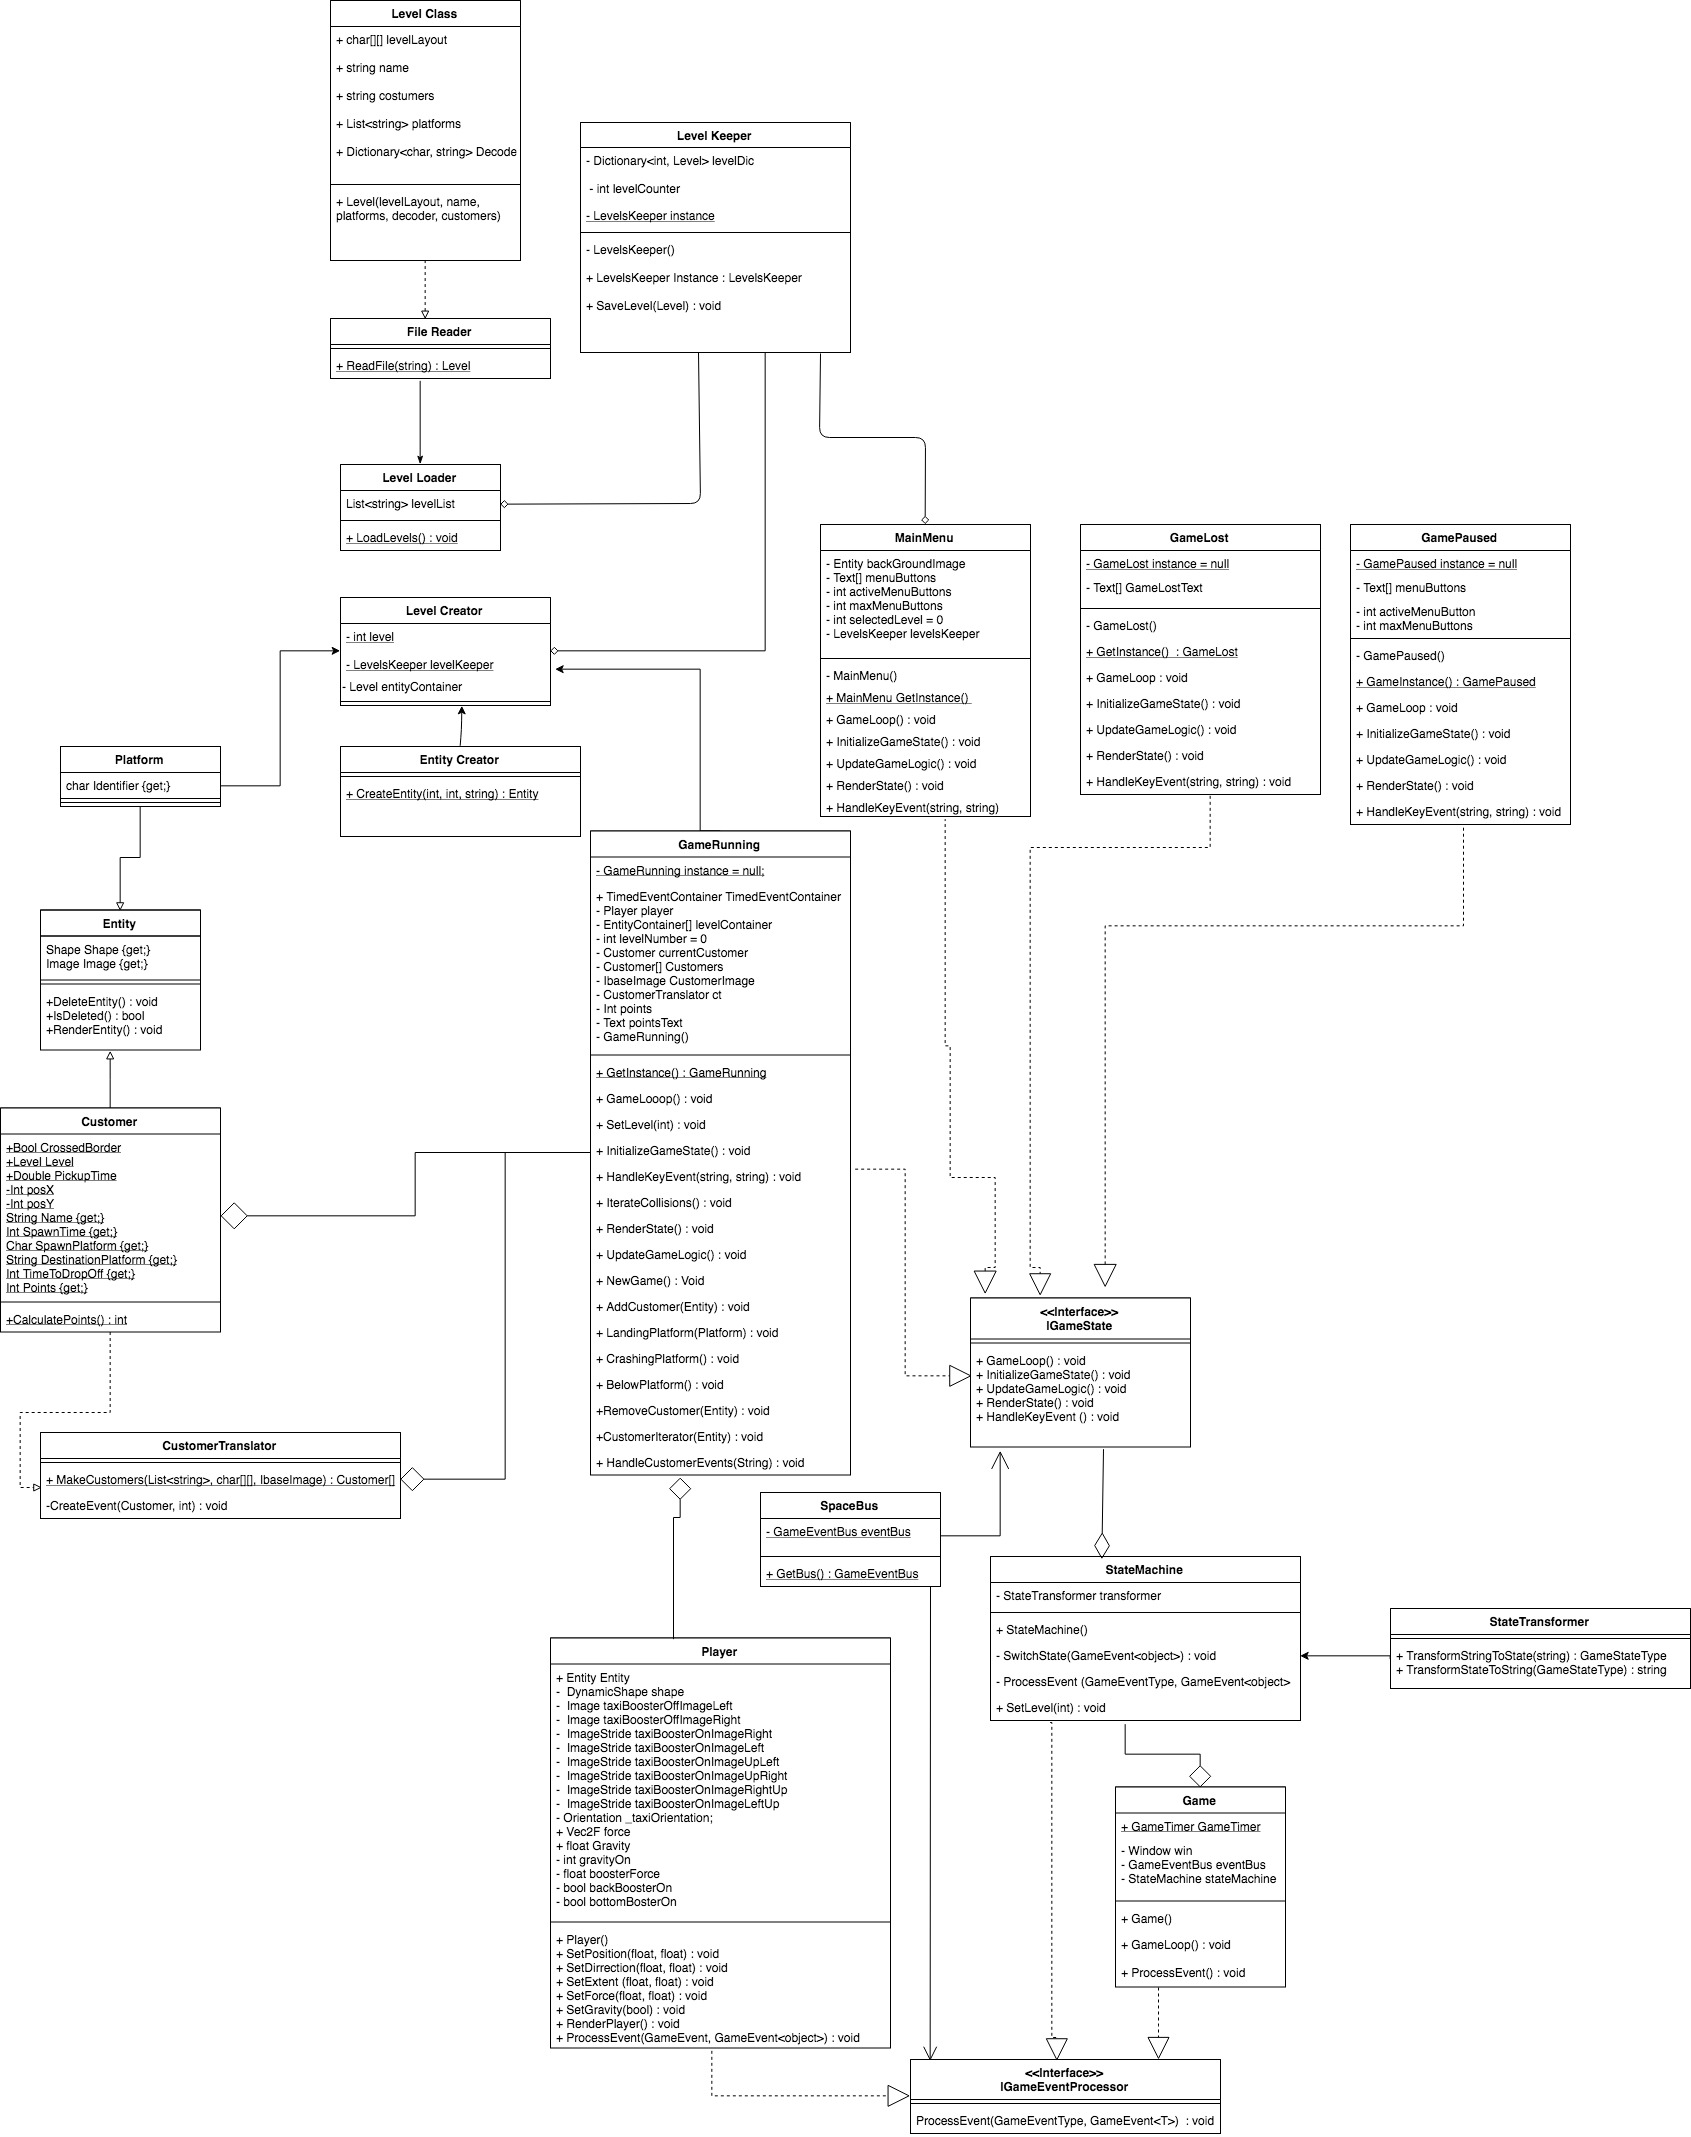
\includegraphics[height=19.3cm]{latex/Images/UML_SU10.jpg}

Selvom flere af vores klasser kun benyttes en gang i programmet har vi valgt at lade dem være konkrete klasser. Da Vi ikke ser nogen grund til at indføre et singleton pattern hos alle klasserne da der ikke sker noget ved at have flere objekter af for eksempel FileReader, så har vi valgt kun at benytte det på udvalgte klasser såsom LevelsKeeper.\\
Da vi ønsker at benytte vores Level objekter som en måde at lagre information om vores levels, har vi valgt kun at implementere en konstruktor til dem og ellers gemme alle informationer i public properties uden setters. Dette garanterer at når Level først er blevet instantieret kan dens informationer ikke overskrives, men informationerne kan til enhver tid læses.\\
LevelsKeeper fungerer som en database for vores levels, og indeholder en dictionary af level numre som keys og Level objekter som values. LevelsKeeper er implementeret som en singleton. Dette er gjort da vi ikke ønsker at have flere 'halve' databaser med kun en delmængde af vores levels. Vi vil dog have et problem hvis der skrives og læses til det samme sted i hukommelsen samtidigt da vi arbejder med referencer. Men som det fremgik af vores sequence diagram vil dette ikke kunne lade sig gøre med den nuværende implementation, men skulle det blive nødvendigt at udvide vores model med endnu en klasse som skriver til LevelsKeeper samtidigt med at spillet kører, så så skal der implementeres en form for sikkerhed imod dette.\\
At LevelsKeeper er en singleton bevirker at både LevelLoader og LevelCreator skal holde en variabel for LevelsKeeper objektet, som kan kalde sin private metode til at gemme et Level objekt, eller kan benytte sin public property til at returnere et level hvis den er givet et indeks. Metoden er privat, og propertien har ingen setter for at følge princippet om at hver class udfører opgaverne for sit eget ansvar.

\subsection{States og StateMachine}
For at gøre det muligt at håndtere vidt forskellige tilstande i spillet, har vi implementeret en state machine. Denne har til opgave at sørge for der bliver skiftet mellem vores states korrekt. Vores implementerede states består af GameRunning som håndterer selve spillet, MainMenu som håndterer vores menu, GamePaused som sørger for at spillet kan pauses og GameLost som fortæller spilleren at spillet er slut. Der er forskellige krav til hvornår der der skal skiftes fra hvilket state til hvilken state, og derfor har StateMachine ansvaret for at kunne tage den rette beslutning om dette. For eksempel skal spillet pauses når spilleren klikker på escape, derfor skal vores EventBus fortælle StateMachine at der er klikket på escape, og StateMachine sørger derefter for at skifte tilstanden til GamePaused. Vi finder også at når spillet tabes, altså når spilleren for eksempel støder ind i en blok, så bedes vores EventBus om at udsende en besked om at skifte tilstanden til GameLost. Der kan altså være flere forskellige måder at skifte tilstanden på hvilket viser at StateMachine er fleksibel.

\subsection{Kollision}
Vi har lavet collision detection i denne opgave, her har det været nødvendigt at kende forskel på om man er stødt ind i en blok eller en platform. Dette har vi gjort ved at når LevelCreator kaldes returnerer den et array af EntityContainers, som GameRunning da kan rendere og lave collision detection på. Collision detection foregår først på index 0 i arrayet af EntityContainers som består af alle platformene, det vil sige at hvis der er kollision her ved vi at man har ramt en platform, og vi kan da fortsætte med de nødvendige efterfølgende checks. Derefter checker den næste index, som består af alle blokkene, hvis en af disse rammes slutter spillet. Hvis der ikke er kollision i nogle af de to EntityContainers tjekkes det om Taxien er over toppen af skærmen, hvis dette er tilfældet ved vi at man er fløjet gennem hullet i toppen af skærmen og næste level loades. I starten havde vi overvejet om vi skulle lave to klasser der arvede fra Entity, hvor den ene klasse kan beskrive en blok, og den anden en platform. Hvis vi havde gjort dette kunne vi nøjes med én EntityContainer der består af både bloks og platforme, vi ville da kunne tjekke typen af den Entity der er stødt ind i. Denne implementation ville dog kræve at vi tjekker typen af det objekt der er stødt ind i, dermed have if-statements der tjekker typen, dette ville være et brud på Open/Close princippet \footnote{Kilde: SU18-B4-03-Design\_Patterns, undervisningsmateriale}. Til excercise 10 har vi alligevel valgt at indføre en platform class da vi er nødsaget til at kunne identificere hvilken platform vi lander på når vi flyver med en customer. Men da vores originale design fungerer valgte vi at fortsætte med dette således at vi ikke skal til at typetjekke og bryde med open/close princippet.\\

\subsection{Fysik}
   En væsentlig del af SpaceTaxi er fysikken i spillet. Denne har vi valgt at integrere med spilleren da vi ved at der ikke vil være andre objekter som skal benytte den. Vi vælger altså at se fysikken i spillet som den måde spilleren skal bevæge sig på, og der er derfor stadig player objektets ansvar at kunne bevæge sig korrekt.\\
   Vi har implementeret tyngdekraften således at vi kan tænde og slukke den. Dette skyldes at når spilleren lander på en platform, så ønsker vi ikke at den skal falde igennem platformen. Derfor slukker vi for tyngdekraften og spillerens fart sættes til nul (forudsat at den ikke dør på grund af en for hård landing eller dårlig vinkel). Tyngdekraften tændes dernæst først igen når rumskibet letter fra platformen. Vi oplever dog at rumskibet kan falde igennem platforme hvis den laver små hop. Vi mistænker dette skyldes at der ikke bliver foretaget collision detection hvis rumskibet bevæger sig meget langsomt, men det er ikke lykkedes os verificere dette.

\subsection{Customers}
   Vores timedevents bliver processed i GameRunning hvilket vi har valgt for at gøre det enklere at spawne customers hvilket vil fremstå om lidt. En customer er en instans af Customer, og indeholder information om den enkelte customer. Den information i LevelsKeeper om hver enkel customer bliver sendt igennem CustomerTranslator som sørger for at vi kan instantiere en customer instans. Vores customers bliver ikke spawnet med det samme spillet startes, og de gemmes derfor i et field i GameRunning. Når der bliver oprettet en customer instans, så bliver der også lavet en timedEvent således at denne customer på et tidspunkt bliver spawnet. Når Denne event triggers, så hives den specifikke customer ned i EntityContainer, som bliver renderet, og på denne måde sørger vi for at vores customers først bliver renderet når de spawnes.\\
   Gennem collisiondetection kan vi finde ud af om en customer bliver ramt af taxien, og hvis det er tilfældet, så sættes et field i denne customer til tidspunktet for kollisionen, og den fjernes fra den EntityContainer som render customers. Når taxien senere kollidere med den korrekte platform så udregner den hentede customer hvor mange points spilleren skal have baseret på hvor lang tid spilleren har været om at afsætte denne customer. Disse points bliver lagt til de allerede eksisterende points som er gemt i GameRunning, og GameRunning kan blot render noget tekst for at indikere pointsummen.\\

\subsection{GamePaused}
   Vi har lavet en funktion der gør man kan pause spillet, men det har ikke været muligt at pause den timer der holder øje med hvornår Customers skal spawne og hvor længe de har været i taxien. Dette skyldes at den timer der er er statisk, og den bruges både til at holde styr på timed events og til at holde øje med hvornår der skal tegnes en ny frame. Det vil sige at man ikke kan sætte timed events på pause uden at stoppe hele flowet i programmet,og det vil derfor ikke være muligt at starte spillet igen. Så hvis man pauser spillet vil tiden stadig gå i spillet og kunderne kan derfor stadig blive ''utålmodige'' mens spillet er pauset. Vi processerer dog kun timed events så længe at spillet kører, det betyder at hvis man har spillet pauset på det tidspunkt hvor kunden burde spawnes, vil denne blot spawne idet man starter spillet igen. 
